
\documentclass[11pt]{article}

\usepackage{listings}
\usepackage{graphicx}
\usepackage{amsmath}
\usepackage{amsfonts}
\usepackage{amssymb}
\usepackage{pgfgantt}
\usepackage{amsthm}
\usepackage{fancyhdr}
\usepackage{rotating}
\usepackage[graphicx]{realboxes}
\renewcommand{\vec}{\bm}
\usepackage{dsfont}
\usepackage{xcolor}
\usepackage{sectsty}
\usepackage[paper=a4paper,top=0.58in,left=1.65in, right=1.65in, bottom=1.65in]{geometry}

\definecolor{lightorange}{RGB}{251,211,168}
\definecolor{darkred}{RGB}{153,0,0}
\definecolor{darkgreen}{RGB}{0,51,25}

\sectionfont{\fontsize{12}{15}\selectfont}
%\usepackage{ifpdf}
  %\ifpdf
    %  \usepackage[pdftex]{graphicx}   % to include graphics
      %\pdfcompresslevel=9
      %\usepackage[pdftex,     % sets up hyperref to use pdftex driver
         %     plainpages=false,   % allows page i and 1 to exist in the same document
            %  breaklinks=true,    % link texts can be broken at the end of line
      %        colorlinks=true,
       %       pdftitle=My Document
        %      pdfauthor=My Good Self
            % ]{hyperref}
   %   \usepackage{thumbpdf}
 % \else
  %    \usepackage{graphicx}       % to include graphics
   %   \usepackage{hyperref}       % to simplify the use of \href
 % \fi



%%%%%%%%%%%%%%%%%%%%%%%%%%%%%%%%%%%
% radix:
% not: $\neg$
% and: $\land$
%  fraction:
% potenza:

\title{ 
\includegraphics[width=\linewidth]{header.png}~
\\[0.5cm]
  \huge{Bachelor Project} \\
\textbf{\Large{Barycentric Data Visualization for Triangle Meshes}}}
\date{Spring Semester 2018}
\author{Costanza \textbf{Volpini} \\ \textcolor{gray}{costanza.volpini@usi.ch} \\ \\ Professor: Kai \textbf{Hormann} \\ Assistant: Jan \textbf{Svoboda}}
\begin{document}
\pagestyle{fancy}
\rhead{\bfseries  Costanza Volpini}
\lhead{\bfseries  Project Proposal}
\maketitle
\newgeometry{paper=a4paper,margin=1.65in}

%%%%%%%
\section{Linear Interpolation}
\section{Extend Flat Shading}
\section{Gaussian Curvature}
\begin{figure}[!htb]
    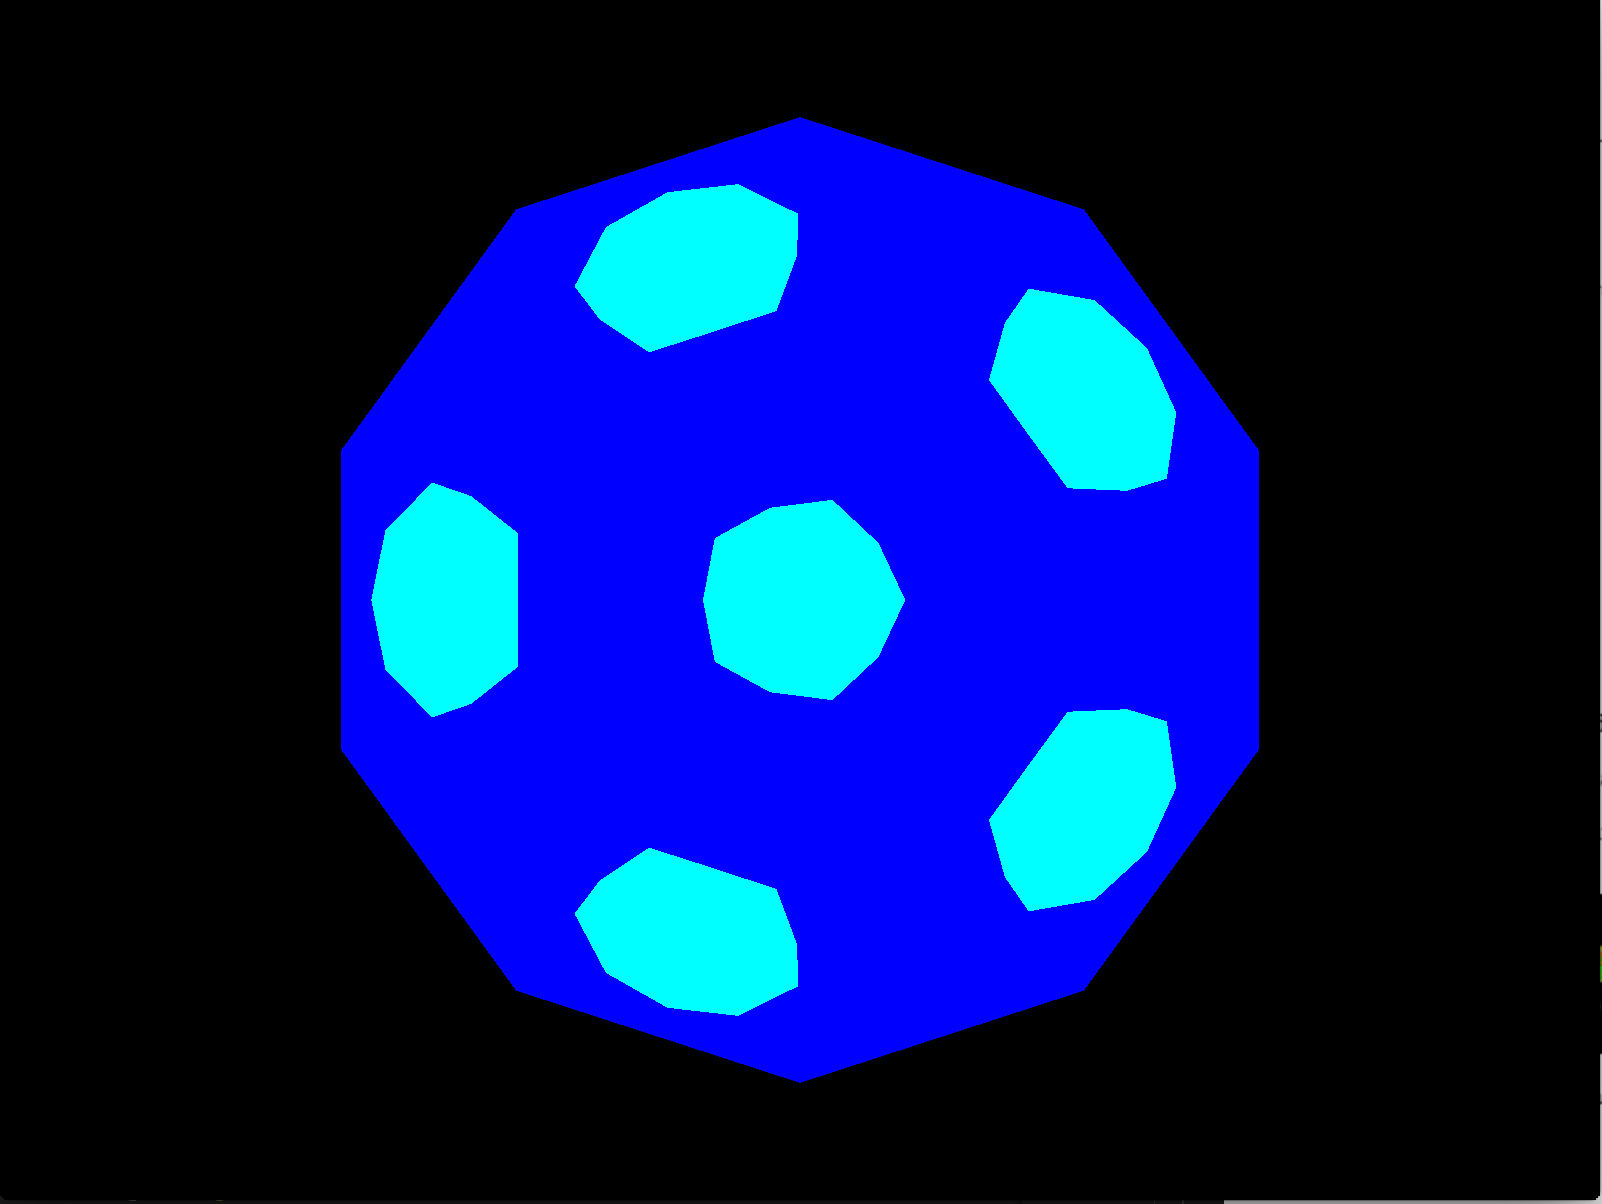
\includegraphics[width=\linewidth]{gaussian-ball.png}
    \caption{Gaussian Curvature}\label{fig:gaussian-ball}
  \end{figure}
\section{Evaluation and comparison}
\begin{figure}[!htb]
  % \minipage{0.32\textwidth}
  %   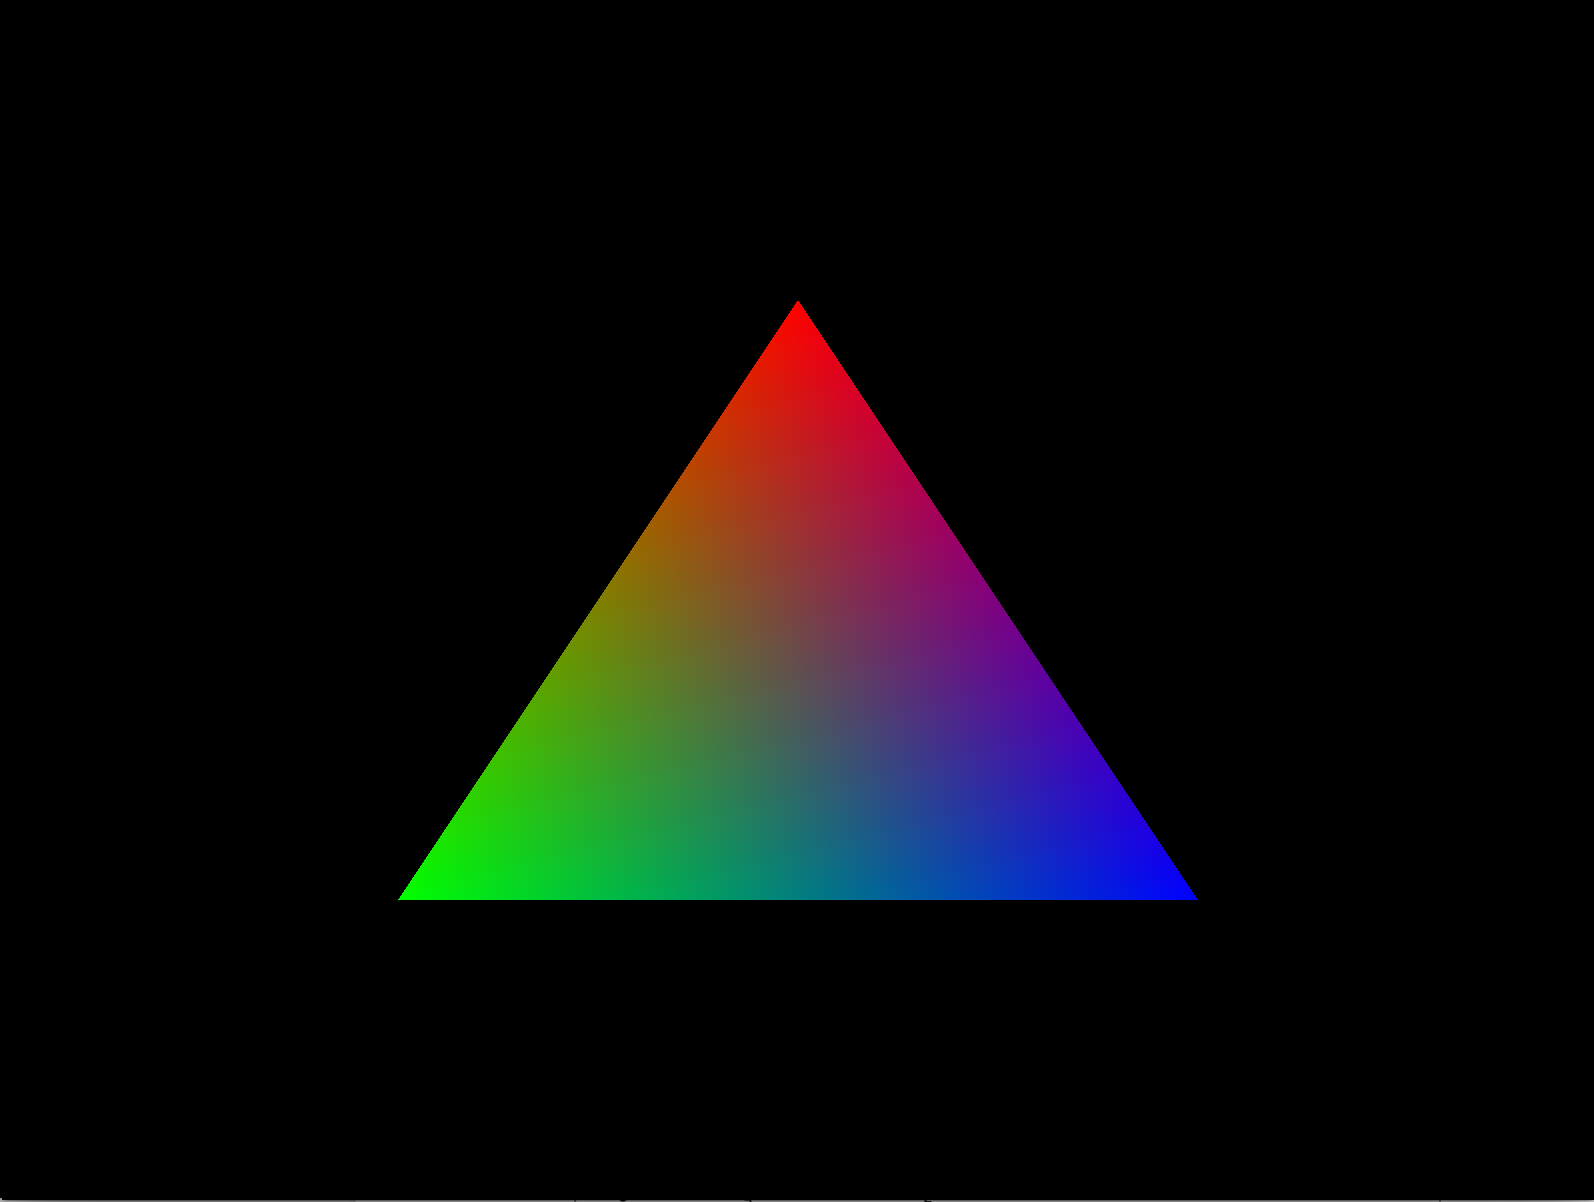
\includegraphics[width=\linewidth]{interpolation.png}
  %   \caption{Interpolation.}\label{fig:interpolation}
  % \endminipage\hfill
  % \minipage{0.32\textwidth}
  %   \includegraphics[width=\linewidth]{flat.png}
  %   \caption{Min Diagram.}\label{fig:min}
  % \endminipage\hfill
  \minipage{0.32\textwidth}%
    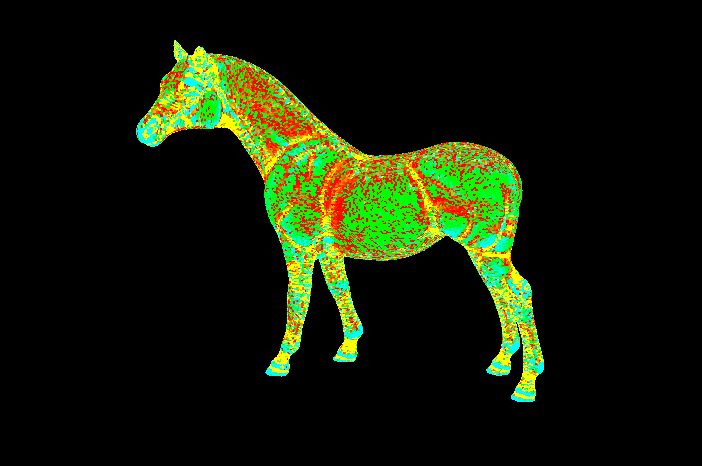
\includegraphics[width=\linewidth]{gaussian.png}
    \caption{Gaussian Curvature}\label{fig:gaussian-horse}
  \endminipage
  \end{figure}

% Using the power of barycentric coordinates we can figure out to which area a pixel belongs and which
% color it should be painted with.

% Passing barycentric coordinates to the fragment shader will clearly demonstrate that we can get results different from the classic
% color interpolation (Fig.\ref{fig:interpolation}).
% \begin{figure}[!htb]
%   \minipage{0.32\textwidth}
%     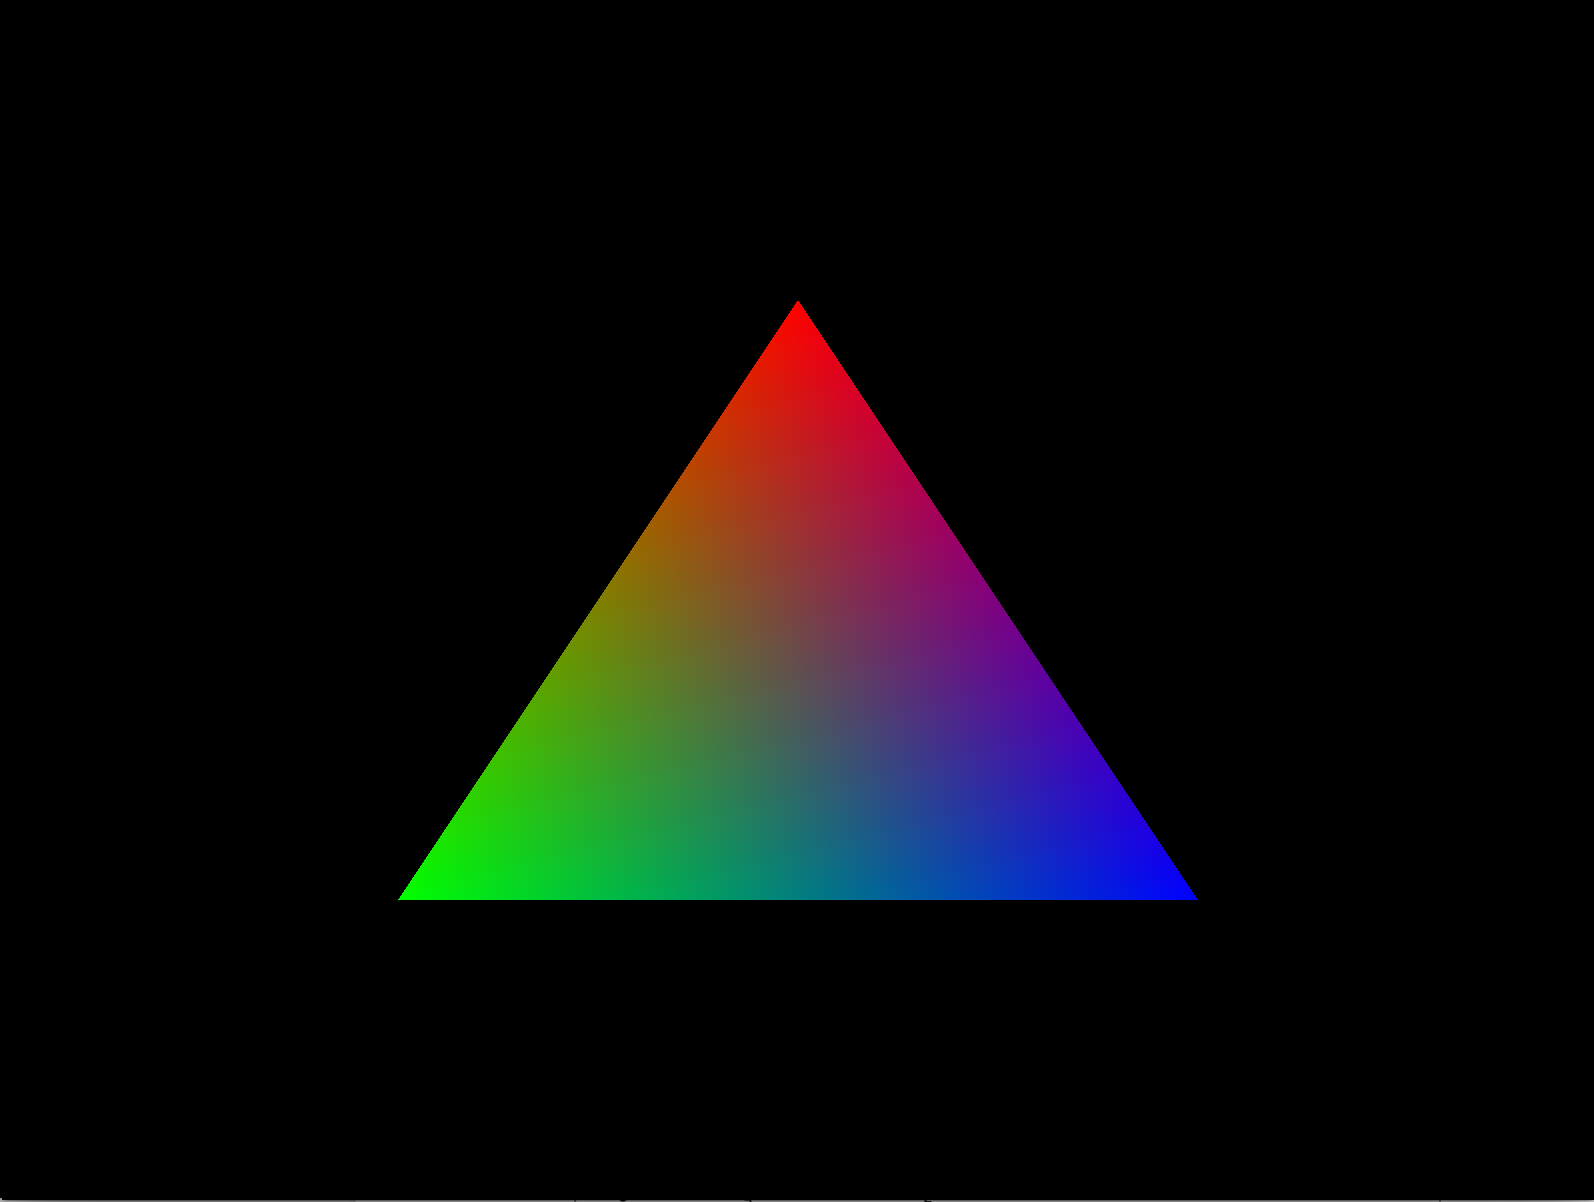
\includegraphics[width=\linewidth]{interpolation.png}
%     \caption{Interpolation.}\label{fig:interpolation}
%   \endminipage\hfill
%   \minipage{0.32\textwidth}
%     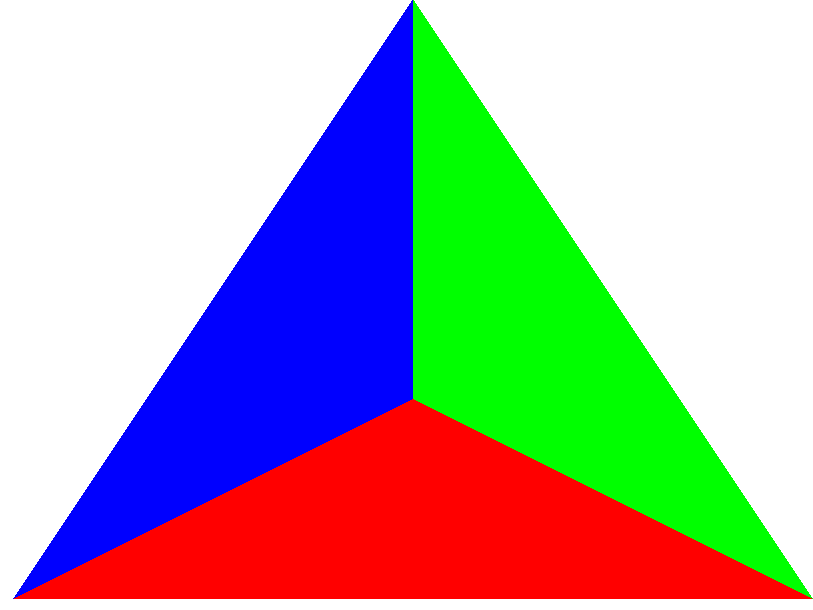
\includegraphics[width=\linewidth]{min.png}
%     \caption{Min Diagram.}\label{fig:min}
%   \endminipage\hfill
%   \minipage{0.32\textwidth}%
%     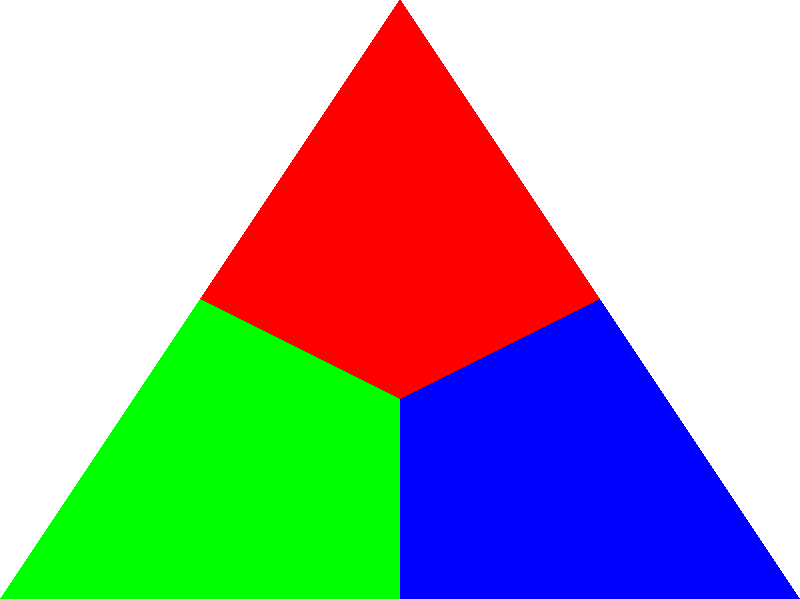
\includegraphics[width=\linewidth]{max.png}
%     \caption{Max Diagram.}\label{fig:max}
%   \endminipage
%   \end{figure}

% vec3(0.001839, -0.029033, 0.004951) mettere questo come valore della matrice per fare la foto


\end{document}

